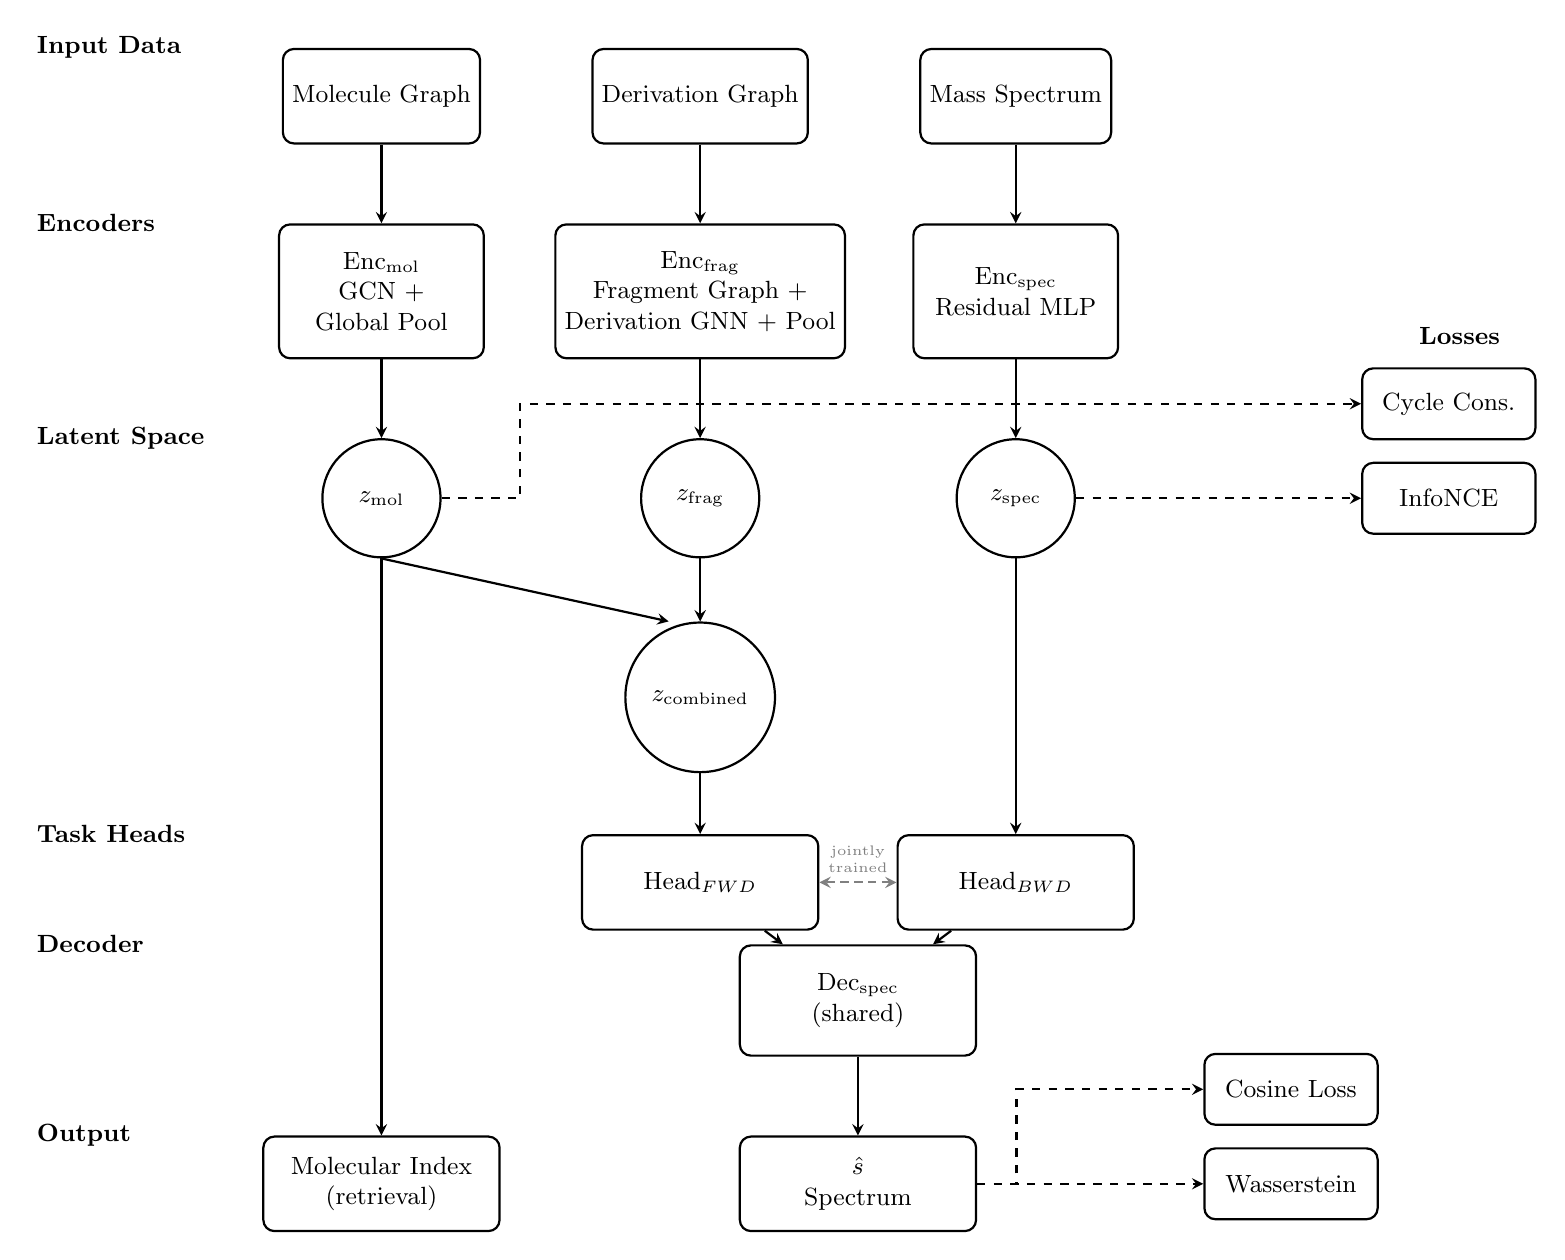
\begin{tikzpicture}[
  node distance = 10mm and 14mm,
  >=stealth,
  inputNode/.style    ={rectangle, rounded corners, draw=black, thick, minimum width=2.2cm, minimum height=1.2cm, text centered, align=center, font=\small},
  encoderNode/.style  ={rectangle, rounded corners, draw=black, thick, minimum width=2.6cm, minimum height=1.7cm, text centered, align=center, font=\small},
  latentNode/.style   ={circle, draw=black, thick, minimum width=1.5cm, text centered, align=center, font=\small},
  headsNode/.style    ={rectangle, rounded corners, draw=black, thick, minimum width=3.0cm, minimum height=1.2cm, text centered, align=center, font=\small},
  decoderNode/.style  ={rectangle, rounded corners, draw=black, thick, minimum width=3.0cm, minimum height=1.4cm, text centered, align=center, font=\small},
  lossNode/.style     ={rectangle, rounded corners, draw=black, thick, minimum width=2.2cm, minimum height=0.9cm, text centered, align=center, font=\small},
  outputNode/.style   ={rectangle, rounded corners, draw=black, thick, minimum width=3.0cm, minimum height=1.2cm, text centered, align=center, font=\small},
  arrow/.style        ={->, thick},
  dashedArrow/.style  ={dashed, ->, thick},
  syncArrow/.style    ={<->, densely dashed, thick, gray},
  groupLabel/.style   ={font=\bfseries\small, anchor=west}
]
\usetikzlibrary{positioning, calc}

% ---- shift the MAIN pipeline right (tune xshift as you like) ----
\begin{scope}[xshift=18mm]

% Define fixed x-coordinate for all labels
\coordinate (labelX) at (-45mm, 0);

% ================== INPUT ROW ==================
\node[inputNode] (MOL)  {Molecule Graph};
\node[inputNode, right=of MOL] (FRAG) {Derivation Graph};
\node[inputNode, right=of FRAG] (SPEC) {Mass Spectrum};
\node[groupLabel] at (labelX |- MOL.north) {Input Data};

% ================== ENCODER ROW ==================
\node[encoderNode, below=of MOL]  (EncMol) {$\mathrm{Enc}_{\mathrm{mol}}$\\GCN +\\Global Pool};
\node[encoderNode, below=of FRAG] (FragSetEnc) {$\mathrm{Enc}_{\mathrm{frag}}$\\Fragment Graph +\\Derivation GNN + Pool};
\node[encoderNode, below=of SPEC] (EncSpec) {$\mathrm{Enc}_{\mathrm{spec}}$\\Residual MLP};
\node[groupLabel] at (labelX |- EncMol.north) {Encoders};

\draw[arrow] (MOL) -- (EncMol);
\draw[arrow] (FRAG) -- (FragSetEnc);
\draw[arrow] (SPEC) -- (EncSpec);

% ================== LATENT ROW ==================
\node[latentNode, below=of EncMol]     (ZM) {$z_{\mathrm{mol}}$};
\node[latentNode, below=of FragSetEnc] (ZF) {$z_{\mathrm{frag}}$};
\node[latentNode, below=of EncSpec]    (ZS) {$z_{\mathrm{spec}}$};

\node[latentNode, minimum width=1.9cm, below=8mm of ZF] (ZFUSED) {$z_{\mathrm{combined}}$};
\node[groupLabel] at (labelX |- ZM.north) {Latent Space};

\draw[arrow] (EncMol) -- (ZM);
\draw[arrow] (FragSetEnc) -- (ZF);
\draw[arrow] (EncSpec) -- (ZS);

% fan-in (avoid stacking)
\draw[arrow] (ZM.south) -- ($(ZFUSED.north)+(-4mm,0)$);
\draw[arrow] (ZF.south) -- (ZFUSED.north);

% ================== HEADS ROW (LogVars removed) ==================
\node[headsNode, below=35mm of ZF] (HdFwd) {Head$_{FWD}$};
\node[headsNode, below=35mm of ZS]  (HdBwd) {Head$_{BWD}$};
\node[groupLabel] at (labelX |- HdFwd.north) {Task Heads};

\draw[arrow] (ZFUSED) -- (HdFwd);
\draw[arrow] (ZS) -- (HdBwd);
\draw[syncArrow] (HdFwd) -- (HdBwd) node[midway, above, font=\tiny, gray, align=center] {jointly\\trained};

% ================== DECODER ROW (single shared spectrum decoder) ==================
\node[decoderNode] (DecSpec) at ($(HdFwd)!0.5!(HdBwd)+(0,-15mm)$) {$\mathrm{Dec}_{\mathrm{spec}}$\\(shared)};
\node[groupLabel] at (labelX |- DecSpec.north) {Decoder};

% both task heads feed the single shared spectrum decoder
\draw[arrow] (HdFwd) -- (DecSpec);
\draw[arrow] (HdBwd) -- (DecSpec);

% ================== OUTPUT ROW ==================
\node[outputNode, below=of DecSpec] (SPEC_HAT) {$\hat{s}$\\Spectrum};

\draw[arrow] (DecSpec) -- (SPEC_HAT);

\end{scope} % end pipeline shift

% ================== INDEX (ALIGNED WITH MOL COLUMN) ==================
\node[outputNode, at=(MOL |- SPEC_HAT)] (INDEX) {Molecular Index\\(retrieval)};
\node[groupLabel] at (labelX |- INDEX.north) {Output};

\draw[arrow] (ZM.south) -- (INDEX.north);

% ================== LOSSES (POSITIONED ON THE RIGHT) ==================
% Position losses in a column to the right of the main diagram
\node[lossNode] at ($(SPEC_HAT)+(55mm,12mm)$) (LOSS_COS)  {Cosine Loss};
\node[lossNode] at ($(SPEC_HAT)+(55mm,0mm)$)  (LOSS_WASS) {Wasserstein};
%\node[lossNode] at ($(SPEC_HAT)+(55mm,-12mm)$) (LOSS_FORB) {Forbidden};
\node[lossNode] at ($(ZS)+(55mm,0mm)$)        (LOSS_CON)  {InfoNCE};
\node[lossNode] at ($(LOSS_CON)+(0mm,12mm)$)   (LOSS_CYCLE){Cycle Cons.};

\node[groupLabel] at ($(LOSS_CYCLE.north)+(-5mm,4mm)$) {Losses};

% Non-overlapping dashed connections
\draw[dashedArrow] (SPEC_HAT.east) -- ++(5mm,0) |- (LOSS_COS.west);
\draw[dashedArrow] (SPEC_HAT.east) -- ++(5mm,0) |- (LOSS_WASS.west);
%\draw[dashedArrow] (SPEC_HAT.east) -- ++(5mm,0) |- (LOSS_FORB.west);

\draw[dashedArrow] (ZS.east) -- ++(10mm,0) |- (LOSS_CON.west);
\draw[dashedArrow] (ZM.east) -- ++(10mm,0) |- (LOSS_CYCLE.west);

\end{tikzpicture}
